\section{Methods}\label{methods}

Fully dense neural network (NN) architectures, such as the one shown in Figure~\ref{fig:nn-1}, perform a sequence of affine transformations, ${\bold z}_i \leftarrow \boldsymbol\theta_i {\bold x}^{(i)}$, followed by element-wise functional operations, $\sigma({\bold z}_i)$ to introduce non-linearity at each layer; that is, each layer stretches and distorts the underlying space.
\begin{figure}[htbp]
\begin{center}
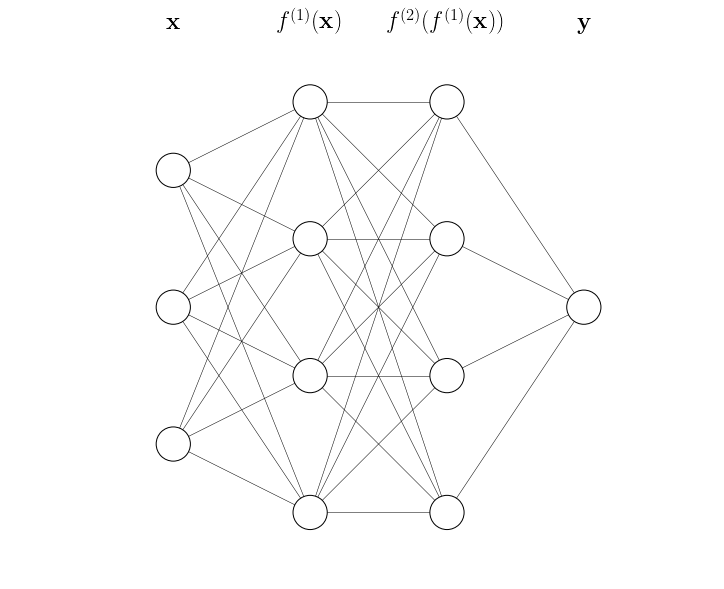
\includegraphics[width=0.4\textwidth]{fig/neural-network-01}
\caption{Schematic view of a fully dense neural network. Each sequence of affine and non-linear transformations are captured in the function, $f_i({\bold x}): {\bold x}^{(i+1)} \leftarrow \sigma(\boldsymbol\theta_i {\bold x}^{(i)})$}
\label{fig:nn-1}
\end{center}
\end{figure}

A typical neural network, as given in (insert neural network reference), is nothing more than an arbitrary function generator, but at present, the network weights can not map back to analytic forms that capture and describe the underlying physics. There are, however, many such mappings through polynomial series expansions (possible reference to other polynomial series expansion applications?). We hypothesize that the physics of a process can be extracted by fitting the polynomial expansions of known physical relationships to the polynomial coefficients of a polynomial series expansion of Equation~(\ref{eqn:nn analytical form}). \\

The goal is to obtain an activation generating function for the chosen activation function in the neural network. There exists many potential options for choosing an activation function such as softplus, softmax, ReLU (rectified linear units), and logistic sigmoid. The details of the derivations for the generating functions of the common activation functions can be found in the appendix. The generating function for the ReLU is dependent on both the input variables and the network weights. Although ReLU (rectified linear units) have become a more common activation function, its discontinuity at $x = 0$ requires an infinite series to fully capture the behavior at this transition. {\color{red}Note: add more pros and cons about each of the common activation functions if necessary}

%\begin{equation}
%	f(x) = log(1+e^x)
%\end{equation}
%
%The series expansion for the exponential
%\begin{equation}
%	e^x = \sum_{k=0}^\infty \frac{x^k}{k!}
%\end{equation}
%where, $a_k = \frac{1}{k!}$, can be expressed as
%\begin{equation}
%	e^x = \sum_{k=0}^\infty x^k a_k
%\end{equation}
%
%A similar series expansion for the logarithm
%\begin{equation}
%	log(1+x) = \sum_{n=1}^\infty (-1)^{n+1} \frac{x^n}{n}
%\end{equation}
%where, $x = e^x$,
%allows for the softplus function to be represented as
%\begin{equation}
%	f(x) = \sum_{n=1}^\infty \frac{(-1)^{n+1}}{n} (\sum_{k=0}^\infty x^k a_k)^n
%\end{equation}
%
%If the expansion of $e^x$ is performed, then it can be seen that
%\begin{equation}
%	(\sum_{k=0}^\infty x^k a_k)^n = (a_0+x(a_1+x(a_2+xa_3...)))^n
%\end{equation}

%Beginning of old softplus derivation and could probably be deleted
%However, the softplus function,
%
%\begin{equation}
%	f(x) = log(1+e^x)
%\end{equation}
%
%The series expansion for the exponential
%\begin{equation}
%	e^x = \sum_{k=0}^\infty \frac{x^k}{k!}
%\end{equation}
%where, $a_k = \frac{1}{k!}$, can be expressed as
%\begin{equation}
%	e^x = \sum_{k=0}^\infty x^k a_k
%\end{equation}
%
%A similar series expansion for the logarithm
%\begin{equation}
%	log(1+x) = \sum_{n=1}^\infty (-1)^{n+1} \frac{x^n}{n}
%\end{equation}
%where, $x = e^x$,
%allows for the softplus function to be represented as
%\begin{equation}
%	f(x) = \sum_{n=1}^\infty \frac{(-1)^{n+1}}{n} 				(\sum_{k=0}^\infty x^k a_k)^n
%\end{equation}
%
%If the expansion of $e^x$ is performed, then it can be seen that
%\begin{equation}
%	(\sum_{k=0}^\infty x^k a_k)^n = 								(a_0+x(a_1+x(a_2+xa_3...)))^n
%\end{equation}
%
%Using the binomial theorem
%\begin{equation}
%	(a+b)^n = \sum_{m=0}^{n} \binom{n}{m} a^{n-m} b^m
%\end{equation}
%where, $a=a_0$ and $b=(x(a_1+x(a_2+xa_3...)))^n$, the series expansion of the exponential can be represented as
%\begin{equation}
%	(\sum_{k=0}^\infty x^k a_k)^n = \sum_{m=0}^{n} 				\binom{n}{m} a_0^{n-m} (a_1+x(a_2+xa_3...))^n x^n
%\end{equation}
%
%Continuing with this approach, it can be seen that ...
%End of old softplus derivation

\subsection{Iterative Determination of ANN Series Expansion Coefficients}
{\color{red}
Any series expansion description of a deep neural network, which is necessarily multilayered, requires a explicit generating function for the coefficients of each layer; a generating function that is a function only of the coefficients of the previous layer and the coefficient generating function of the series expansion of the current layer's activation function.

A derivation for the polynomial expansion coefficient generating function for vector-valued function (layer 1 to layer 2) is presented below, which is an extension of a scalar expansion, provided in \ref{appendix}.}

% {\color{red}
% The element-wise exponent is used repeatedly in both the constitutive relation and neural network expansions. For the product of two matrices, $A: A \in \mathbb{R}^{m \times n}$ and $B: B \in \mathbb{R}^{n \times q}$, the element-wise exponent results in an expanded basis that explicitly includes the cross terms from ${\bf A}$ and ${\bf B}$.
%
% \begin{subequations}
% \begin{align}
%         \left( AB \right)^{\circ p} &= \he[\left( \densematrix{a}{m}{n} \densematrix{b}{n}{q} \right)]{p} \nonumber \\
%             &= \begin{pmatrix}
%                 {\bf a}_{1k}{\bf b}_{k1}  & {\bf a}_{1k}{\bf b}_{k2}    & \cdots    & {\bf a}_{1k}{\bf b}_{kq}   \\
%                 {\bf a}_{2k}{\bf b}_{k1}  & {\bf a}_{2k}{\bf b}_{k2}    &           & \vdots \\
%                 \vdots                    &                             & \ddots    &          \\
%                 {\bf a}_{mk}{\bf b}_{k1}  & \cdots                      &           & {\bf a}_{mk}{\bf b}_{kq}
%             \end{pmatrix}^{\circ p} \nonumber \\
%             &= \begin{pmatrix}
%                 ({\bf a}_{1k}{\bf b}_{k1})^{p}  & ({\bf a}_{1k}{\bf b}_{k2})^{p}    & \cdots    & ({\bf a}_{1k}{\bf b}_{kq})^{p}   \\
%                 ({\bf a}_{2k}{\bf b}_{k1})^{p}  & ({\bf a}_{2k}{\bf b}_{k2})^{p}    &           & \vdots \\
%                 \vdots                          &                                   & \ddots           &          \\
%                 ({\bf a}_{mk}{\bf b}_{k1})^{p}  & \cdots                            &           & ({\bf a}_{mk}{\bf b}_{kq})^{p}
%             \end{pmatrix} \label{eqn:hadmard exponent matrix} \\[3ex]
%         ({\bf a}_{ik}{\bf b}_{kj})^{p} &= (a_{i1}b_{1j} + a_{i2}b_{2j} + \cdots + a_{in}b_{nj})^p \nonumber \\
%             &= \sum_{k1 + k2 + \cdots + k_n = p} \binom{p}{k_1, k_2, \ldots, k_n} \prod_{m=1}^n (a_{im}b_{mj})^{k_m} \nonumber \\
%             &= \sum_{\| {\bf k} \|_1 = p} \binom{p}{k_1, k_2, \ldots, k_n} \prod_{m=1}^n (a_{im}b_{mj})^{k_m} \\%
%     \label{eqn:hadamard exponent vector}
% \end{align}
% \label{eqn:nondistributive hadamard}
% \end{subequations}
% where summation over a repeated index is assumed. That is, Equation~\ref{eqn:hadamard exponent vector} is the expansion of the element-wise exponent of a vector product, $({\bf a}{\bf b})\he{p} = ({\bf a}{\bf b})^p \ne \he[{\bf a}]{p}\he[{\bf b}]{p}$.
% }
%
% % %%%%%%%%%%%%%%%%%%%%%%%%%%%%%%%%%%%%%%%%%%%%%%%%%%%%%%%%%%%%%%%%%%%%%%%%%%%%
% The analytical form, combining Equations~(\ref{eqn:nn analytical form}) and (\ref{eqn:sigmoid zeta expansion}), the estimated output of a two-layer NN can be written as an expansion:
%
% \begin{eqnarray}
% 	{\bold y}_1 & = & \sum_{k=0}^\infty a_k (\boldsymbol\theta_1^T {\bold x})\he{k} \nonumber \\
% 	{\bold y}_2 & = & \sum_{k=0}^\infty b_k (\boldsymbol\theta_2^T {\bold y}_1)\he{k} \nonumber \\
% 		& = & b_0 {\bold 1} + \nonumber\\
% 		&   & + b_1 (\tilde a_0 +%
% 					(\tilde a_1 + %
% 						(\tilde a_2 + %
% 							(\tilde a_3 + %
% 								(\ldots) \tilde {\bold x} )%
% 							\tilde {\bold x} )%
% 						\tilde {\bold x} )%
% 					\tilde {\bold x}) \nonumber \\
% 		&   & + b_2 (\tilde a_0 +%
% 					(\tilde a_1 + %
% 						(\tilde a_2 + %
% 							(\tilde a_3 + %
% 								(\ldots) \tilde {\bold x} )%
% 							\tilde {\bold x} )%
% 						\tilde {\bold x} )%
% 					\tilde {\bold x})^2 \nonumber \\
% 		&   & \vdots \nonumber \\
% 		&   & + b_k (\tilde a_0 +%
% 					(\tilde a_1 + %
% 						(\tilde a_2 + %
% 							(\tilde a_3 + %
% 								(\ldots) \tilde {\bold x} )%
% 							\tilde {\bold x} )%
% 						\tilde {\bold x} )%
% 					\tilde {\bold x})^k \nonumber \\
% 		&   & \vdots
% \end{eqnarray}
% \noindent where $\tilde a_i = \boldsymbol\theta_2^T a_i$ and $\tilde{\bold x} = \boldsymbol\theta_1^T {\bold x}$. All $\boldsymbol\theta_i$, ${\bold x}$, and ${\bold y}$ are augmented to include the bias, ${\bold b}_i$, that is,
% \begin{eqnarray}
% 	{\bold x}&:& {\bold x} \leftarrow \begin{pmatrix}
% 								1 \\
% 								{\bold x}
% 							\end{pmatrix} = \begin{pmatrix}
% 											1 \\
% 											x_0 \\
% 											x_1 \\
% 											\vdots \\
% 											x_n
% 										\end{pmatrix}\\
% 	{\bold y}&:& {\bold y} \leftarrow \begin{pmatrix}
% 								1 \\
% 								{\bold y}
% 							\end{pmatrix} \\
% 	\boldsymbol\theta_i&:& \boldsymbol\theta_i \leftarrow \begin{pmatrix} {\bold b}_i & \boldsymbol\theta_i \end{pmatrix}
% \end{eqnarray}
%
% The element-wise exponent operator, ${\bf x}\he{m} = (x_1^m\ x_2^m\ \cdots\ x_n^m)^T$, raises each element of a vector or matrix to the specified power, $m$.
%
% From Equation~(\ref{eqn:sigmoid zeta expansion}), $a_i  = 0\ \text{for}\ i = 2, 4, 6, \ldots$, and therefore,
% \begin{align}
% 	{\bold y}_1 =& \sum_{k=0}^\infty a_k (\boldsymbol\theta_1^T {\bold x})\he{k} \nonumber \\
% 	{\bold y}_2 =& \sum_{k=0}^\infty b_k (\boldsymbol\theta_2^T {\bold y}_1)\he{k} \nonumber \\
% 		=& b_0 {\bold 1} + \nonumber\\
% 		 &+ b_1 (\tilde a_0 +%
% 					(\tilde a_1 + %
% 						(\tilde a_3 + %
% 							(\tilde a_5 + %
% 								(\ldots) \tilde {\bold x}\he{2} )%
% 							\tilde {\bold x}\he{2} )%
% 						\tilde {\bold x}\he{2} )%
% 					\tilde {\bold x}) \nonumber \\
% 		&+ b_2 (\tilde a_0 +%
% 					(\tilde a_1 + %
% 						(\tilde a_3 + %
% 							(\tilde a_5 + %
% 								(\ldots) \tilde {\bold x}\he{2} )%
% 							\tilde {\bold x}\he{2} )%
% 						\tilde {\bold x}\he{2} )%
% 					\tilde {\bold x})\he{2} \nonumber \\
% 		& \vdots \nonumber \\
% 		& + b_k (\tilde a_0 +%
% 					(\tilde a_1 + %
% 						(\tilde a_3 + %
% 							(\tilde a_5 + %
% 								(\ldots) \tilde {\bold x}\he{2} )%
% 							\tilde {\bold x}\he{2} )%
% 						\tilde {\bold x}\he{2} )%
% 					\tilde {\bold x})\he{k} \nonumber \\
% 		& \vdots \nonumber \\
% 	{\bold y}_2 = & \sum_{N=0}^\infty \sum_{k=0}^{N} \sum_{l=0}^{k} \sum_{m=0}^{l} \ldots %
% 		b_N %
% 		\binom{N}{k,l,m,\ldots} %
% 		\tilde a_0^k \tilde a_1^l \tilde a_3^m \ldots %
% 		\tilde {\bold x}\he{(N-k\ldots)} %
% 		({\tilde {\bold x}^2})\he{(N-k-l\ldots)} %
% 		({\tilde {\bold x}^2})\he{(N-k-l-m\ldots)} \nonumber \\
% 	 =& \sum_{N=0}^\infty \sum_{k=0}^{N} \sum_{l=0}^{k} \sum_{m=0}^{l} \ldots %
% 		b_N %
% 		\binom{N}{k,l,m,\ldots} %
% 		\tilde a_0^k \tilde a_1^l \tilde a_3^m \ldots %
% 		\tilde {\bold x}\he{(l+m+n+\ldots)} %
% 		({\tilde {\bold x}\he{2}})\he{(m+n+\ldots)} %
% 		({\tilde {\bold x}\he{2}})\he{(n+\ldots)}
% 	\label{eqn:ANN power series coefficient generating function}
% \end{align}
% \noindent where $k+l+m+n+\ldots = N$. Collecting coefficients and terms of power $k$,
% \begin{equation*}
% 	{\bold y_2} =  \sum_{k=0}^\infty c_k \tilde{\bold x}\he{k}
% \end{equation*}
% \noindent that, having the same form as Equation~(\ref{eqn:sigmoid zeta expansion}) creates a sequential process for determining the coefficients of the power series expansion of each layer in an ANN. Importantly, the output layer in a ANN regression is a single node with a linear activation, so the final layer, $y_f$, working from the last hidden layer, ${\bold y}_n$, is simply,
% \begin{equation}
% 	y_f = \boldsymbol\theta_n^T {\bold y}_n
% \end{equation}

%Beginning of scalar coefficients derivation.%
\subsection{Polynomial Expansion of a Scalar Layer}
\label{sec:polynomial series scalar}

We can represent the recursive structure of an ANN as a series of transformations on a particular power series. Using this method, we are able to write an algorithm that will compute the coefficients of a power series determined by some ANN up to an arbitrary order of approximation.\\

For the sake of illustration, we present the next derivation in terms of a simplified ANN with one neuron in each layer. For the treatment of a unsimplified ANN, see Appendix.

\subsubsection{Notation}
Suppose that $x \in \mathbb{R}$ is a scalar, $y \in \mathbb{R}$ is a scalar, $\theta \in \mathbb{R}$ is a scalar, and $\sigma: \mathbb{R} \to \mathbb{R}$ is an analytic function. Since $\sigma$ is analytic, it can be represented as

\begin{align}
    \sigma(x)
    &= s_0 + s_1 x + s_2 x^2 + \cdots \nonumber \\
	&= \sum_{k=0}^{\infty} s_{k} x^{k}.
	\label{eqn:scalar layer activation}
\end{align}

Suppose that we can represent $x$ as a power series of another scalar $z$.

\begin{align}
    x
    &= a_0 + a_1 z + a_2 z^2 + \cdots \nonumber \\
	&= \sum_{n=0}^{\infty} a_{n} z^{n}.
	\label{eqn:scalar x series}
\end{align}

Finally, suppose that we have the relation

\begin{equation}
	y = \sigma(\theta x).
	\label{eqn:scalar layer relation}
\end{equation}

This represents a single-neuron layer of an ANN with input $x$, weight $\theta$, output $y$, and activation $\sigma$. The value of $z$ can be intrepreted as the input to the entire ANN.

\subsubsection{Objective}
Similarly, $y$ can also be represented as a power series with $b_i$ for $i = 0, 1, 2, \ldots$ as the coefficient using the same approach. We will rewrite the relation for $y$ given by Equation (\ref{eqn:scalar layer relation}) to find the coefficients $b_i$ for $i = 0, 1, 2, \ldots$ for Equation (\ref{eqn: eqn:scalar y series}).

\begin{align}
    y
    &= \sigma(\theta x) \nonumber \\
    &= \sum_{k=0}^{\infty} s_k (\theta x)^k \nonumber \\
    &= \sum_{k=0}^{\infty} s_k \theta^k \left(\sum_{n=0}^{\infty} a_{n} z^{n}\right)^{k} \nonumber \\
	&= \sum_{k=0}^{\infty} s_k \theta^k \left(\sum_{k_0 + k_1 + k_2 + \cdots = k} \binom{k}{k_0, k_1, k_2, \cdots} \prod_{n=0}^{\infty} (a_n z^{n})^{k_n} \right)
	\label{eqn:scalar y expansion}
\end{align}

Note that we used the multinomial theorem to expand the penultimate term in the equation.

\subsubsection{Coefficient Extraction}

At this point, it is infeasible to attempt to write Equation (\ref{eqn:scalar y expansion}) directly as a power series. Instead, we will extract the coefficients $b_i$ for $i = 0, 1, 2, \ldots$ by observing constraints on the coefficients.\\

First, as a result of the multinomial theorem, we have a constraint on the inner sum in Equation (\ref{eqn:scalar y expansion}), which is constraint on the index of the sum so we shall call this an index constraint.\\

Second, the coefficient $b_i$ is associated with the term $z^i$ so we must form an equality between $i$ and the power on $z$ in Equation (\ref{eqn:scalar y expansion}). To satisfy this equality, a constant is required. This is a constraint on the power of the scalar $z$ so we shall call this a power constraint. This constraint implies $k_{i + 1} = k_{i + 2} = \cdots = 0$. Therefore, both the index constraint and power constraint can be reduced to a finite series instead of an infinite series.

\begin{equation}
	k = \sum_{n=0}^{i} k_n, \qquad i = \sum_{n=0}^{i} n k_n
\end{equation}

If a collection of $k_j$ for $j = 0, 1, 2, \ldots$ satisfy both of these constraints, then, the constant coefficients of $z^i$ may be pulled out and added to the sum of $b_i$. In concise terms we have derived that

\begin{equation}
    b_i = \sum_{k=0}^{\infty} s_k \theta^k \sum_{\substack{k_0 + k_1 + \cdots + k_i = k \\ 0 k_0 + 1 k_1 + \cdots + i k_i = i}} \binom{k}{k_0, k_1, \cdots, k_i} \prod_{n=0}^{\infty} a_n^{k_n}.
	\label{eqn:scalar power series result}
\end{equation}

Thus, we have derived a tractable method of computing the coefficients of a power series after a linear and nonlinear transformation. We have included some worked examples of these coefficients in Appendix \ref{sec:worked scalar coeffs}.
%End of scalar coefficients derivation.%

%If no reference, prove that the primal/dual is unique.
%Weidmann J. (1980) Linear operators and their adjoints. In: Linear Operators in Hilbert Spaces. Graduate Texts in Mathematics, vol 68. Springer, New York, NY
%Riesz representation theorem for proving that the dual is unique???
